% Options for packages loaded elsewhere
\PassOptionsToPackage{unicode}{hyperref}
\PassOptionsToPackage{hyphens}{url}
\PassOptionsToPackage{dvipsnames,svgnames,x11names}{xcolor}
%
\documentclass[
  letterpaper,
  DIV=11,
  numbers=noendperiod,
  oneside]{scrartcl}

\usepackage{amsmath,amssymb}
\usepackage{iftex}
\ifPDFTeX
  \usepackage[T1]{fontenc}
  \usepackage[utf8]{inputenc}
  \usepackage{textcomp} % provide euro and other symbols
\else % if luatex or xetex
  \usepackage{unicode-math}
  \defaultfontfeatures{Scale=MatchLowercase}
  \defaultfontfeatures[\rmfamily]{Ligatures=TeX,Scale=1}
\fi
\usepackage{lmodern}
\ifPDFTeX\else  
    % xetex/luatex font selection
\fi
% Use upquote if available, for straight quotes in verbatim environments
\IfFileExists{upquote.sty}{\usepackage{upquote}}{}
\IfFileExists{microtype.sty}{% use microtype if available
  \usepackage[]{microtype}
  \UseMicrotypeSet[protrusion]{basicmath} % disable protrusion for tt fonts
}{}
\makeatletter
\@ifundefined{KOMAClassName}{% if non-KOMA class
  \IfFileExists{parskip.sty}{%
    \usepackage{parskip}
  }{% else
    \setlength{\parindent}{0pt}
    \setlength{\parskip}{6pt plus 2pt minus 1pt}}
}{% if KOMA class
  \KOMAoptions{parskip=half}}
\makeatother
\usepackage{xcolor}
\usepackage[left=1in,marginparwidth=2.0666666666667in,textwidth=4.1333333333333in,marginparsep=0.3in]{geometry}
\setlength{\emergencystretch}{3em} % prevent overfull lines
\setcounter{secnumdepth}{5}
% Make \paragraph and \subparagraph free-standing
\ifx\paragraph\undefined\else
  \let\oldparagraph\paragraph
  \renewcommand{\paragraph}[1]{\oldparagraph{#1}\mbox{}}
\fi
\ifx\subparagraph\undefined\else
  \let\oldsubparagraph\subparagraph
  \renewcommand{\subparagraph}[1]{\oldsubparagraph{#1}\mbox{}}
\fi


\providecommand{\tightlist}{%
  \setlength{\itemsep}{0pt}\setlength{\parskip}{0pt}}\usepackage{longtable,booktabs,array}
\usepackage{calc} % for calculating minipage widths
% Correct order of tables after \paragraph or \subparagraph
\usepackage{etoolbox}
\makeatletter
\patchcmd\longtable{\par}{\if@noskipsec\mbox{}\fi\par}{}{}
\makeatother
% Allow footnotes in longtable head/foot
\IfFileExists{footnotehyper.sty}{\usepackage{footnotehyper}}{\usepackage{footnote}}
\makesavenoteenv{longtable}
\usepackage{graphicx}
\makeatletter
\def\maxwidth{\ifdim\Gin@nat@width>\linewidth\linewidth\else\Gin@nat@width\fi}
\def\maxheight{\ifdim\Gin@nat@height>\textheight\textheight\else\Gin@nat@height\fi}
\makeatother
% Scale images if necessary, so that they will not overflow the page
% margins by default, and it is still possible to overwrite the defaults
% using explicit options in \includegraphics[width, height, ...]{}
\setkeys{Gin}{width=\maxwidth,height=\maxheight,keepaspectratio}
% Set default figure placement to htbp
\makeatletter
\def\fps@figure{htbp}
\makeatother

\KOMAoption{captions}{tableheading}
\makeatletter
\@ifpackageloaded{caption}{}{\usepackage{caption}}
\AtBeginDocument{%
\ifdefined\contentsname
  \renewcommand*\contentsname{Table of contents}
\else
  \newcommand\contentsname{Table of contents}
\fi
\ifdefined\listfigurename
  \renewcommand*\listfigurename{List of Figures}
\else
  \newcommand\listfigurename{List of Figures}
\fi
\ifdefined\listtablename
  \renewcommand*\listtablename{List of Tables}
\else
  \newcommand\listtablename{List of Tables}
\fi
\ifdefined\figurename
  \renewcommand*\figurename{Figure}
\else
  \newcommand\figurename{Figure}
\fi
\ifdefined\tablename
  \renewcommand*\tablename{Table}
\else
  \newcommand\tablename{Table}
\fi
}
\@ifpackageloaded{float}{}{\usepackage{float}}
\floatstyle{ruled}
\@ifundefined{c@chapter}{\newfloat{codelisting}{h}{lop}}{\newfloat{codelisting}{h}{lop}[chapter]}
\floatname{codelisting}{Listing}
\newcommand*\listoflistings{\listof{codelisting}{List of Listings}}
\makeatother
\makeatletter
\makeatother
\makeatletter
\@ifpackageloaded{caption}{}{\usepackage{caption}}
\@ifpackageloaded{subcaption}{}{\usepackage{subcaption}}
\makeatother
\makeatletter
\@ifpackageloaded{sidenotes}{}{\usepackage{sidenotes}}
\@ifpackageloaded{marginnote}{}{\usepackage{marginnote}}
\makeatother
\ifLuaTeX
  \usepackage{selnolig}  % disable illegal ligatures
\fi
\usepackage{bookmark}

\IfFileExists{xurl.sty}{\usepackage{xurl}}{} % add URL line breaks if available
\urlstyle{same} % disable monospaced font for URLs
\hypersetup{
  pdftitle={Telling Stories With Data: Graphing Change Over Time},
  pdfauthor={Andy Grogan-Kaylor},
  colorlinks=true,
  linkcolor={blue},
  filecolor={Maroon},
  citecolor={Blue},
  urlcolor={Blue},
  pdfcreator={LaTeX via pandoc}}

\title{Telling Stories With Data: Graphing Change Over Time}
\author{Andy Grogan-Kaylor}
\date{2024-02-19}

\begin{document}
\maketitle

\renewcommand*\contentsname{Table of contents}
{
\hypersetup{linkcolor=}
\setcounter{tocdepth}{3}
\tableofcontents
}
\section{Graphs}\label{graphs}

\subsection{Scatterplot}\label{scatterplot}

We start in thinking about graphing change over time with a
scatterplot.\sidenote{\footnotesize Scatterplots show every data point. However, with
  many data points, scatterplots may become overcomplicated, and
  difficult to interpret. Points may even be plotted over other data
  points.} \sidenote{\footnotesize Note that we are using \emph{color} and \emph{line
  type} to distinguish different individuals. This may not always be
  possible, especially when there are a large number of individuals in
  the data.}

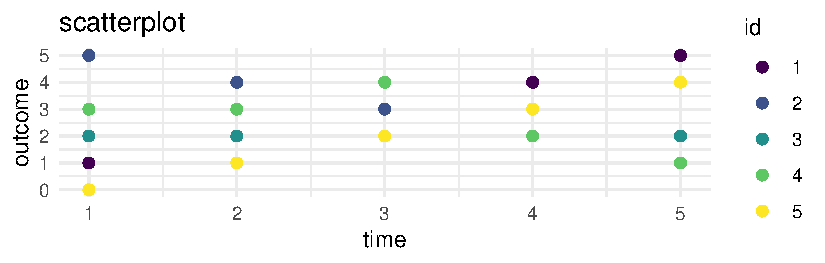
\includegraphics{index_files/figure-pdf/unnamed-chunk-1-1.pdf}

\subsection{Line Plot}\label{line-plot}

A natural next step is to connect the dots of a scatterplot with
straight line segments to form a line plot. \sidenote{\footnotesize With any of the
  options discussed, one may consider \emph{small multiples} where each
  individual trajectory is placed in its own sub-graph.}

\marginnote{\begin{footnotesize}

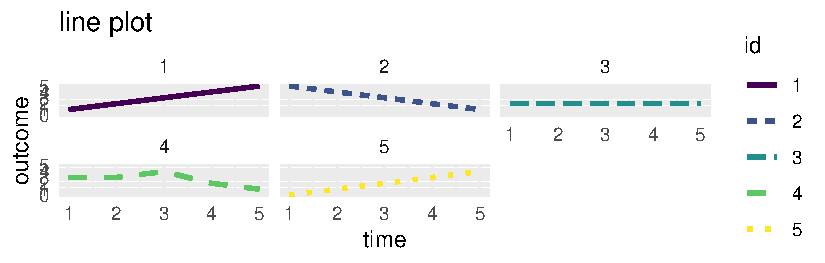
\includegraphics{index_files/figure-pdf/unnamed-chunk-2-1.pdf}

\end{footnotesize}}

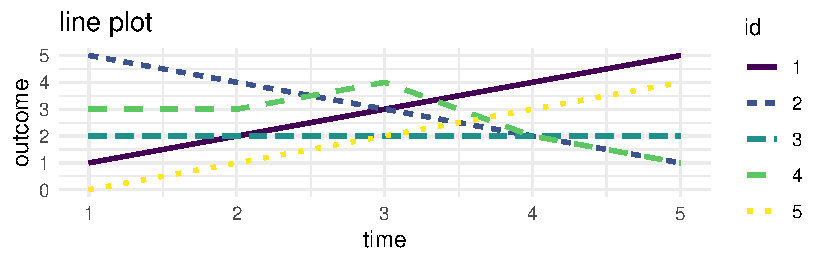
\includegraphics{index_files/figure-pdf/unnamed-chunk-3-1.pdf}

\subsection{Spaghetti Plot}\label{spaghetti-plot}

Instead of simply connecting the observations, one may estimate an
individual linear trajectory. In \emph{multilevel modeling} these line
plots showing individual estimated linear trajectories are sometimes
called \emph{spaghetti plots}.

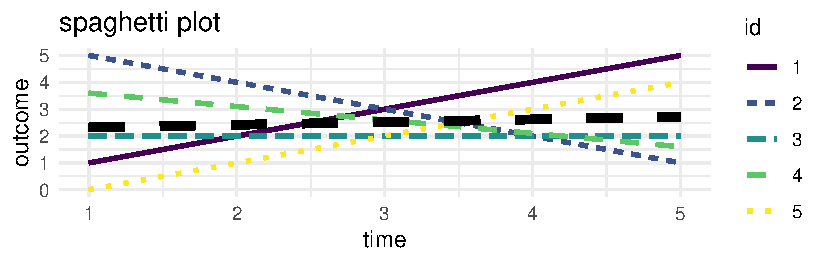
\includegraphics{index_files/figure-pdf/unnamed-chunk-4-1.pdf}

\subsection{Smoothed Trajectories}\label{smoothed-trajectories}

Alternatively, rather than connecting observations with straight lines,
or estimating an overall straight line trajectory for each individual,
it may be useful to \emph{smooth} the trajectories by drawing curved
lines between individual observations.\sidenote{\footnotesize One needs to be careful,
  however, as the smoothed trajectories may give the impression of
  having more data points than one actually has.}

\marginnote{\begin{footnotesize}

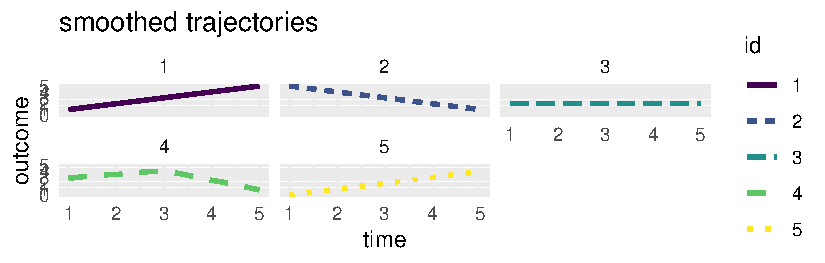
\includegraphics{index_files/figure-pdf/unnamed-chunk-5-1.pdf}

\end{footnotesize}}

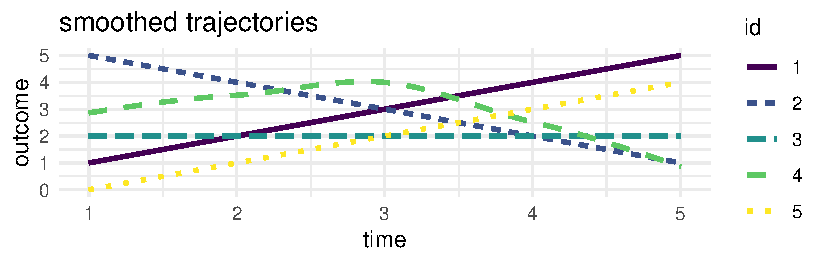
\includegraphics{index_files/figure-pdf/unnamed-chunk-6-1.pdf}

\subsection{Slopegraph}\label{slopegraph}

An increasingly popular option is a slope graph.\sidenote{\footnotesize In order to be
  clear and effective, a slope graph may often only show the outcome at
  the beginning point, and at the end point. A slope graph may be less
  satisfactory when there are multiple timepoints. The small multiple
  idea works with a slopegraph as well.}

\marginnote{\begin{footnotesize}

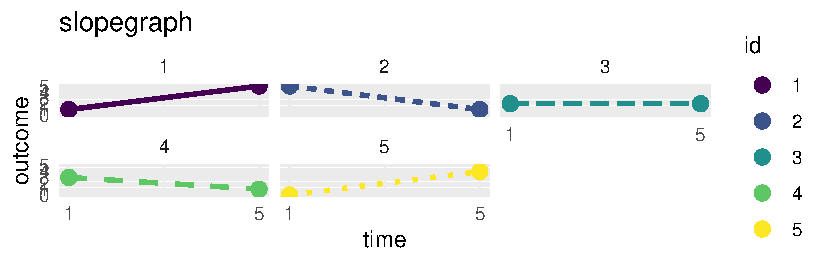
\includegraphics{index_files/figure-pdf/unnamed-chunk-7-1.pdf}

\end{footnotesize}}


\includegraphics{index_files/figure-pdf/unnamed-chunk-8-1.pdf}

\section{The Data Used In This Example Are
Simulated.}\label{the-data-used-in-this-example-are-simulated.}

\marginnote{\begin{footnotesize}

\begin{marginfigure}

{\centering 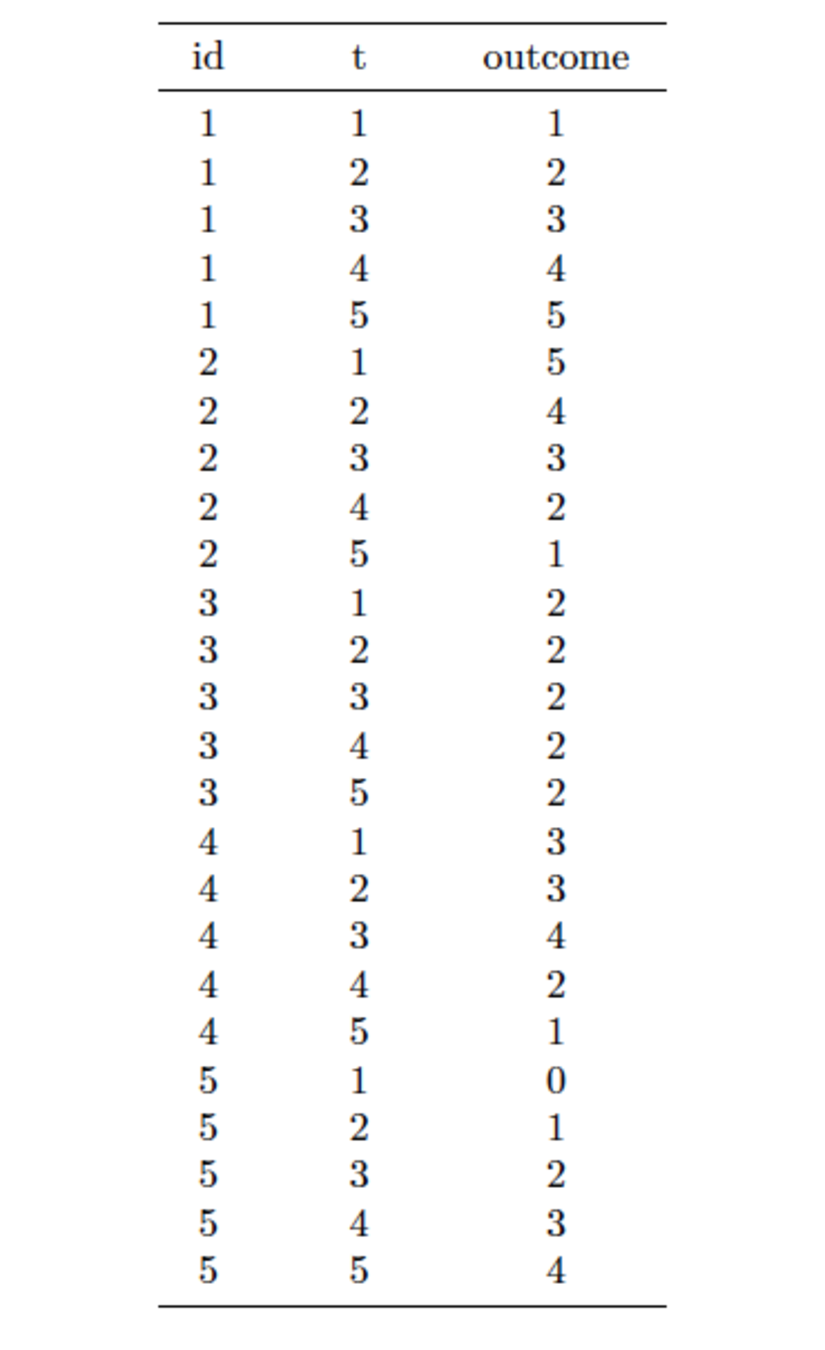
\includegraphics{index_files/figure-pdf/unnamed-chunk-9-1.pdf}

}

\caption{Long Data}

\end{marginfigure}%

\end{footnotesize}}

Many data sets, but not all, are originally created in the \emph{wide}
format--as shown below--where every row of data is an \emph{individual},
and an individual only has a \emph{single row}. Ideally, every row in
\emph{wide} data is uniquely identified by an individual \emph{id}
number.

\begin{longtable}[]{@{}
  >{\centering\arraybackslash}p{(\columnwidth - 10\tabcolsep) * \real{0.0694}}
  >{\centering\arraybackslash}p{(\columnwidth - 10\tabcolsep) * \real{0.1667}}
  >{\centering\arraybackslash}p{(\columnwidth - 10\tabcolsep) * \real{0.1667}}
  >{\centering\arraybackslash}p{(\columnwidth - 10\tabcolsep) * \real{0.1667}}
  >{\centering\arraybackslash}p{(\columnwidth - 10\tabcolsep) * \real{0.1667}}
  >{\centering\arraybackslash}p{(\columnwidth - 10\tabcolsep) * \real{0.1667}}@{}}
\toprule\noalign{}
\begin{minipage}[b]{\linewidth}\centering
id
\end{minipage} & \begin{minipage}[b]{\linewidth}\centering
outcome.1
\end{minipage} & \begin{minipage}[b]{\linewidth}\centering
outcome.2
\end{minipage} & \begin{minipage}[b]{\linewidth}\centering
outcome.3
\end{minipage} & \begin{minipage}[b]{\linewidth}\centering
outcome.4
\end{minipage} & \begin{minipage}[b]{\linewidth}\centering
outcome.5
\end{minipage} \\
\midrule\noalign{}
\endhead
\bottomrule\noalign{}
\endlastfoot
1 & 1 & 2 & 3 & 4 & 5 \\
2 & 5 & 4 & 3 & 2 & 1 \\
3 & 2 & 2 & 2 & 2 & 2 \\
4 & 3 & 3 & 4 & 2 & 1 \\
5 & 0 & 1 & 2 & 3 & 4 \\
\end{longtable}

Generally, for graphing change over time, it is most appropriate to have
data that are in a \emph{long} format, as shown in the margin. In
\emph{long} data every row represents a particular \emph{measurement
occasion} for a \emph{particular individual}. Each individual in the
data set thus has \emph{multiple rows}. Ideally, every row in data in
the \emph{long} format is uniquely identified by the combination of an
\emph{id} number and a \emph{study wave}.

Data can be \emph{reshaped} from \emph{wide} to \emph{long} format, and
\emph{vice versa}. Two straightforward options are the \texttt{reshape}
command, as available in both \href{http://www.stata.com}{Stata} and
\href{https://www.r-project.org/}{R}.

\footnotesize

Graphics made with \href{http://ggplot2.org/}{ggplot2}created by Hadley
Wickham.



\end{document}
